\documentclass[tikz,border=10pt]{standalone}
\PassOptionsToPackage{dvipsnames}{xcolor}

\usepackage{tikz}
\usepackage{pifont}

\renewcommand*\familydefault{\sfdefault}

\definecolor{nodecolor}{RGB}{83, 98,158}
\usetikzlibrary{shapes,positioning,arrows.meta,quotes,backgrounds}
\begin{document}
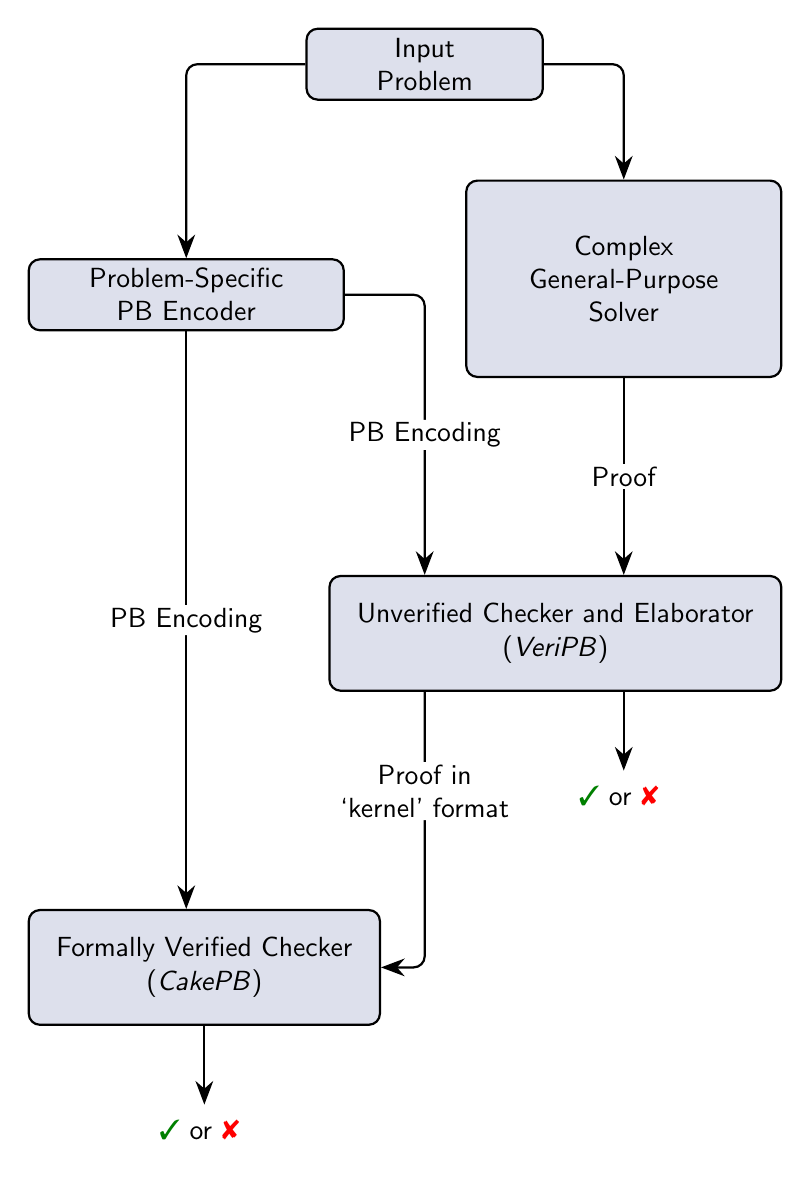
\begin{tikzpicture}[
    every node/.style = {draw, fill=nodecolor!20, align=center, rounded corners},
    every path/.append style = {draw, -{Stealth[length=3mm]}, thick, rounded corners},
    label/.style = {text=black, draw=none,fill=white,inner sep=1pt}]

    % INPUT
    \node [inner xsep = 1em, minimum width=3cm ] (input) at (0, 2) {Input\\Problem};

    % SOLVER
    \node [below right = 1cm and -1cm of input, minimum width=4cm, inner ysep=2em ]
    (solver) {Complex\\General-Purpose\\Solver};

    % ENCODER
    \node [below left = 2cm and -0.5cm of input, minimum width=4cm ] (encoder)
    {Problem-Specific\\PB Encoder};

    % CHECKER
    \node [below=2.5cm of solver.south east, anchor=north east, inner sep = 1em]
    (checker) {Unverified Checker and Elaborator\\(\textit{VeriPB})};

    % VERIFIED CHECKER
    \coordinate (checkerbottomleft) at (encoder.west|-checker.south);
    \coordinate (checkerbottomright) at (solver.south|-checker.south);
    \node [inner sep = 1em, below=3.5cm of checkerbottomleft, anchor=west]
    (verifiedchecker) {Formally Verified Checker\\(\textit{CakePB})};

    % RESULT FROM CHECKER
    \node [inner sep = 0.5em, draw=none, fill=white, below=1cm of checkerbottomright]
    (result1) { \textcolor{green!50!black}{\ding{51}} or \textcolor{red}{\ding{56}} };

    % RESULT FROM VERIFIED CHECKER
    \node [inner sep = 0.5em, draw=none, fill=white, below=1cm of verifiedchecker]
    (result2) { \textcolor{green!50!black}{\ding{51}} or \textcolor{red}{\ding{56}} };

    % ARROWS AND LABELS
    \draw (input) -| (solver);

    \draw (input) -| (encoder);

    \draw (encoder) -| node[pos=0.75,draw,label] {PB Encoding} (checker.north-|input);

    \draw (solver.south) -- node[label] {Proof} (solver.south|-checker.north);

    \draw (encoder) -- node[label] {PB Encoding} (encoder|-verifiedchecker.north);

    \draw (checkerbottomright) -- (result1);

    \draw (verifiedchecker) -- (result2);

    \draw (checker.south-|input) |- node[pos=0.18,label] {Proof in\\`kernel' format}
    (verifiedchecker);
\end{tikzpicture}

\end{document}